
\section{Figures and Tables}

    \subsection{Figures}
		
    	\figref{fig:figure} shows a 3D surface plot of the hyperbolic paraboloid $z=x^2-y^2$.
    		
    	\begin{figure}[H]
    		\centering
    		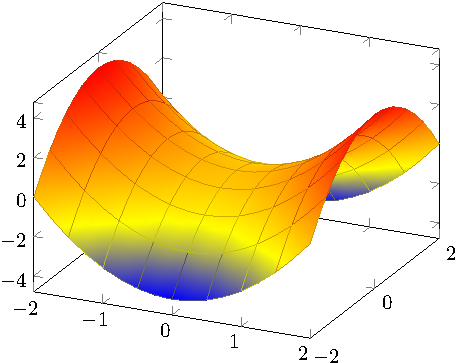
\includegraphics[width=0.75\columnwidth]{figures/Example.pdf}
    		\caption{Hyperbolic paraboloid obtained from PGFPlots \cite{PFGPlots}.}
    		\label{fig:figure}
    	\end{figure}

    \subsection{Tables}
	
        \tabref{tab:table} shows an example table of some astronomical objects. 

        \begin{table}[H]
        	\caption{Astronomical Object Data}
        	\label{tab:table}
        	\begin{tabular}{
        		>{\raggedright\arraybackslash}p{0.25\columnwidth}
        		>{\raggedright\arraybackslash}p{0.30\columnwidth}
        		>{\raggedright\arraybackslash}p{0.31\columnwidth}
        	}
        	\toprule
        	\textbf{Object} & \textbf{Type} & \textbf{Distance (Light Years)} \\
        	\midrule
        	Alpha Centauri & Star system & 4.37 \\
        	Betelgeuse & Red supergiant star & 642.5 \\
        	Andromeda & Spiral galaxy & 2.537 million \\
        	Earth & Planet & 0 \\
        	Sirius & Binary star system & 8.6 \\
        	\bottomrule
        	\end{tabular}
        	\tabletext{Note: The table contains data of some famous celestial objects.}
        \end{table}

        The \inlinecode{\tabletext{}} command is used to add notes to tables easily. 

